\documentclass[border=6pt]{standalone}
\usepackage{tikz}
\usetikzlibrary{arrows.meta}
\begin{document}
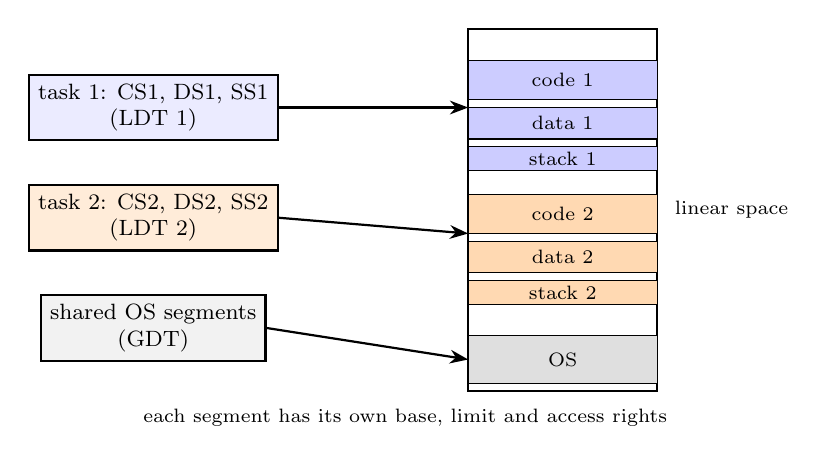
\begin{tikzpicture}[>=Stealth,font=\small]
\node[draw,thick,fill=blue!8,font=\footnotesize,align=center,minimum width=2.6cm] (t1) at (0,1.0) {task 1: CS1, DS1, SS1\\(LDT 1)};
\node[draw,thick,fill=orange!15,font=\footnotesize,align=center,minimum width=2.6cm] (t2) at (0,-0.4) {task 2: CS2, DS2, SS2\\(LDT 2)};
\node[draw,thick,fill=gray!10,font=\footnotesize,align=center,minimum width=2.6cm] (os) at (0,-1.8) {shared OS segments\\(GDT)};
\draw[thick] (4.0,2.0) rectangle (6.4,-2.6);
\foreach \y/\h/\c/\t in {1.6/0.5/blue!20/code 1,1.0/0.4/blue!20/data 1,0.5/0.3/blue!20/stack 1,-0.1/0.5/orange!30/code 2,-0.7/0.4/orange!30/data 2,-1.2/0.3/orange!30/stack 2,-1.9/0.6/gray!25/OS} {
  \draw[fill=\c] (4.0,\y) rectangle (6.4,\y-\h);
  \node[font=\scriptsize] at (5.2,\y-\h/2) {\t};
}
\draw[->,thick] (t1.east) -- (4.0,1.0);
\draw[->,thick] (t2.east) -- (4.0,-0.6);
\draw[->,thick] (os.east) -- (4.0,-2.2);
\node[font=\scriptsize,anchor=west] at (6.5,-0.3) {linear space};
\node[font=\scriptsize,anchor=north,align=center] at (3.2,-2.7) {each segment has its own base, limit and access rights};
\end{tikzpicture}
\end{document}
